\begin{tikzpicture}
\node[inner sep=0pt] (obrazek) at (0,0)
    {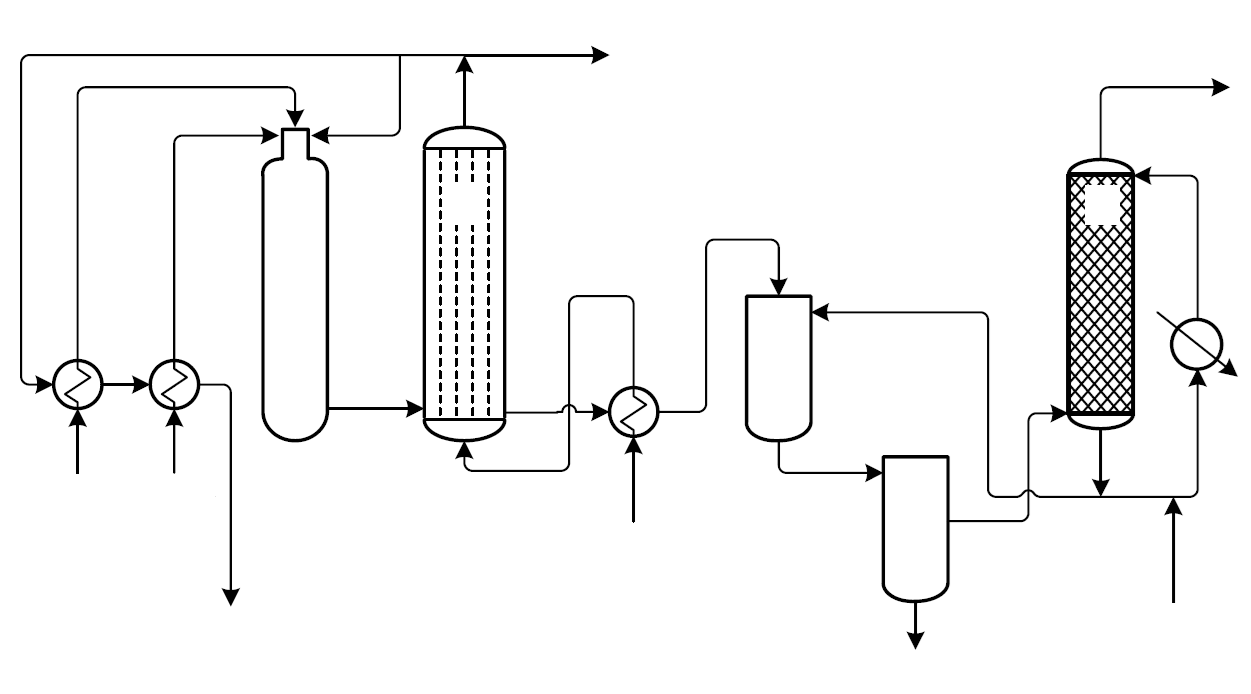
\includegraphics[width=0.8\textwidth]{figures/schema_pox.png}};
\node[font=\small\bfseries] at (-2.95,1.3) {1};
\node[font=\small\bfseries] at (-1.45,1.3) {2};
\node[font=\small\bfseries] at (1.36,0.1) {3};
\node[font=\small\bfseries] at (2.6,-1.4) {4};
\node[font=\small\bfseries] at (4.27,1.26) {5};

\node[font=\scriptsize,align=center] at (-4.9,-1.6) {těžký\\olej};
\node[font=\scriptsize] at (-4,-1.44) {kyslík};
\node[font=\scriptsize] at (-3.5,-2.55) {kondenzát};
\node[font=\scriptsize] at (-4,2.85) {vysokotlaká pára};
\node[font=\scriptsize] at (1.1,2.625) {vysokotlaká pára};
\node[font=\scriptsize,align=center] at (1.05,1.35) {surový\\plyn};
\node[font=\scriptsize,align=center] at (0.05,-1.95) {napájecí\\voda};
\node[font=\scriptsize] at (2.6,-2.9) {sazová voda};
\node[font=\scriptsize] at (4.9,-2.55) {voda};
\node[font=\scriptsize] at (5.1,1.75) {voda};
\node[font=\scriptsize] at (2.5,0.53) {voda};
\node[font=\scriptsize] at (4.4,2.6) {surový plyn};
\end{tikzpicture}